\documentclass[journal]{IEEEtran}
\usepackage{graphicx}
\graphicspath{{../}}
\pagestyle{empty}
\raggedbottom
\begin{document}
\typeout{REDESIGN-TEXTWIDTH=\the\textwidth}
\typeout{REDESIGN-COLUMNWIDTH=\the\columnwidth}
\twocolumn[{
\centering
{\small NeST-Com: figures 2 and 3, actual-size review}\par\vspace{3mm}
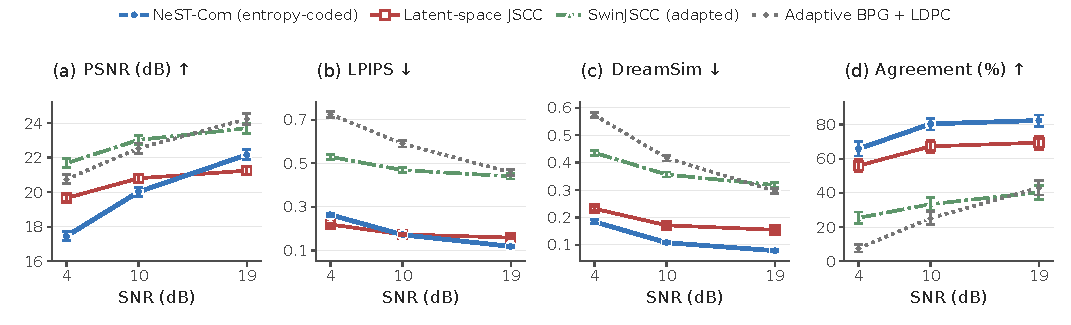
\includegraphics[width=\textwidth]{fig2_main_1x4.pdf}\par
\begin{minipage}{\textwidth}\footnotesize
Fig. 2. Reconstruction performance at $N=1024$ on the original common500 images. Markers show source-averaged means and error bars show pointwise 95\% source-level bootstrap intervals after averaging three channel realizations per source. The entropy-coded method uses the corrected m10-enabled policy at 19\,dB. Latent-space JSCC and adapted SwinJSCC use their final 100k and 200k checkpoints. SNR is numerically spaced; prediction agreement is not label accuracy.
\end{minipage}\par\vspace{7mm}
}]
\noindent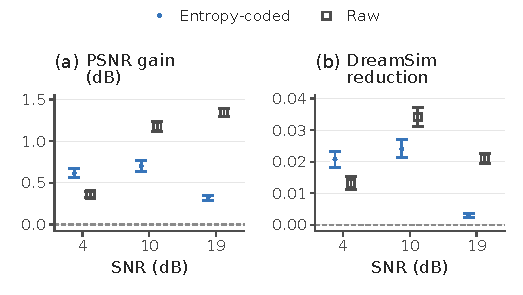
\includegraphics[width=\columnwidth]{fig3_paired_two_panels.pdf}\par
\noindent{\footnotesize\raggedright Fig. 3. Paired effects of within-scale truncation on common500 at $N=1024$, evaluated separately for raw and entropy-coded source representations. Positive values indicate higher PSNR or lower DreamSim. Intervals are direct pointwise 95\% source-paired bootstrap intervals after three-noise averaging. The entropy-coded 19\,dB comparison includes m10 in both families. Horizontal positions are categorical operating points; the two series are offset for clarity. Original family-specific MCS settings are retained.\par}
\vspace{5mm}
\noindent{\footnotesize\raggedright Review only: original manuscript widths; figures included without further scaling. Figure 2: 181.3533$\times$55\,mm. Figure 3: 88.5679$\times$50\,mm. Print this PDF at 100\% (disable fit-to-page). No new experiments, scoring, or bootstrap. Full captions and provenance accompany the figures.\par}
\end{document}
